\section{Conjoncture et politiques économiques} % (fold)
\label{prt:conjoncture_et_politiques_economiques}

Les différents organismes économiques réalisent des prévisions de taux de croissance du PIB. Mais leurs prévisions divergent de fait des modèles utilisés et 
des hypothèses réalisées.
L'approche macroéconomique de cette section, se base sur l'\emph{analyse de Keynes} 
et la \emph{synthèse néoclassique} ensuite opérée. 
On étudiera les \emph{modèles IS-LM} qui permettent donc de prévoir
les variations du PIB ainsi que l'impact au niveau du \emph{chômage} et de l'\emph{inflation}. 

L'économiste Kaldor propose d'analyser les phénomènes macro à l'aide du ``carré magique''.
Celui-ci est représenté à la Figure~\ref{fig:carre_magique} et on dira que la situation
économique d'un pays est jugée d'autant plus satisfaisante que la surface du quadrilatère
est proche de la situation idéale définie, dans ce cas-ci le carré en bleu.

\begin{figure}[h]
	\begin{center}
		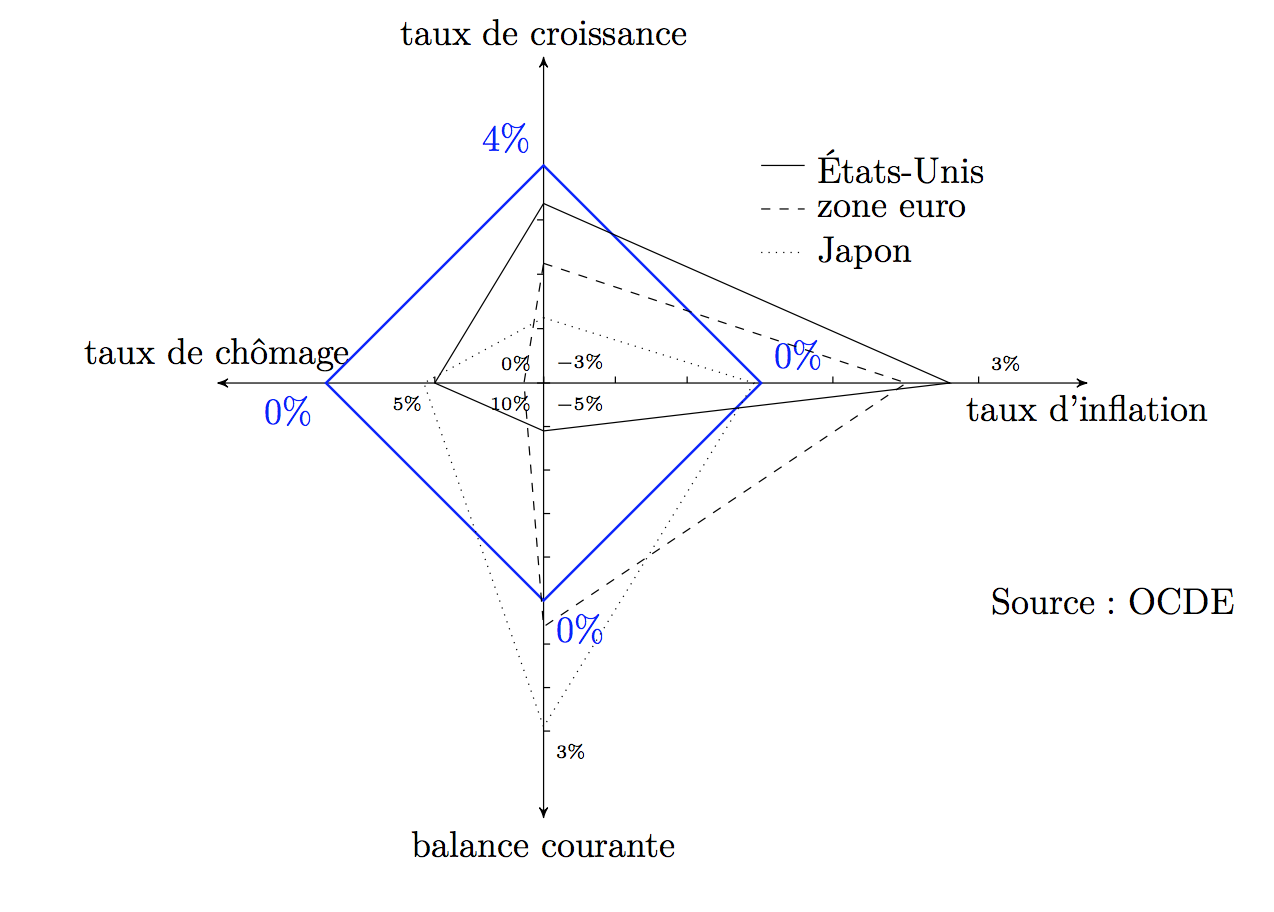
\includegraphics[scale=0.5]{./img/im2}
	\end{center}
	\caption{Carré magique : moyenné de 1996 à 2006}
  \label{fig:carre_magique}
\end{figure}

Les différents axes du \emph{carré magique} représentent les objectifs de la politique macroéconomique. 
On s'intéressera dans ce chapitre aux trois premiers. 
On recueille différentes politiques économiques, chronologiquement discernables comme suit : 
\begin{itemize}[label=\ding{69}]
	\item \emph{Les trente glorieuses (45-73)} : une politique plus simple. 
  Une réponse parfaite à l'analyse keynésienne, en cas de récession et chômage élevé
	on instaurait des politques budgétaires et monétaires expansionnistes (le contraire si chômage faible
  et inflation). On parle de politique de \textsc{Stop and Go}, la représentaiton économique 
  de ce phénomène s'appelle \emph{la courbe de Phillips}.
	\item \emph{À partir de soixante-dix} : on voit apparaître la \emph{stagflation}, c'est-à-dire un
  chômage croissant dans un environnement inflationniste. On retrouve pour cette période deux visions
  sur les fluctuations.
  \begin{enumerate}
    \item Selon les économistes \emph{néo-keynésiens}, l'État doit intervenir pour réguler le marché.
    \item Tandis que selon les \emph{nouveaux classiques}, l'État ne doit pas intervenir car les fluctuations
    sont des réponses naturelles du marché.
  \end{enumerate}
  \item \emph{Seconde partie des parties quatre-vingt} : la lutte contre l'inflation est le principal
  objectif des politiques. Celui-ci est atteint au moyen d'une politique budgétaire restrictive
  qui entraîne des taux presque nuls et des soutiens moindres des gouvernements.
  \item Une poursuite de cette politique restrictive s'est vue causée par 3 éléments principaux : 
  \begin{enumerate}
  	\item Réunification allemande qui présentait un risque inflationniste de fait du fort besoin de financement.
  	\item Mise en oeuvre de l'euro qui devait se présenter comme une monnaie forte.
  	\item Objectif majeur du déficit public imposé aux pays européens.
  \end{enumerate}
  \item Dans l'actualité, on aurait pu se poser la question de la réalisation d'une politique expansioniste. C'est la crise de 2009 qui a poussé cette décision,
  en effet, pour protéger l'emploi. Cependant après une stabilisation, on a vu une déflation apparaître et la BCE à donc décidé de diminuer les taux pour 
  favoriser les investissements et inciter les banques à réaliser des crédits.
\end{itemize}

Mais pourquoi la BCE ? Les États sont trop susceptibles de favoriser des injections dans un cadre démagogique, pré-élections. 

\subsection{Politique monétaire} % (fold)
\label{sub:politique_monetaire}

Kaldor stipule que l'illusion monétaire consistant à avoir une impression de hausse du pouvoir d'achat est grevé par l'inflation. Il n'est donc que purement 
démagogique de réaliser des politiques d'inflation avant des élections. De plus la courbe de Phillips stipulant qu'une hausse du pouvoir d'achat induit 
une baisse du chômage (Figure~\ref{fig:courbe_phillips}) est remise en cause par Friedmann qui stipule que les salariés anticipant l'inflation vont demander une hausse de
leur salaire afin de maintenir constant leur salaire nominal. Cette école classique est celle suivie par la BCE. Les principes de la BCE se qualifient 
d'orthodoxie monétaire car ils consistent à établir une règle crédible et à s'y soumettre. 
\begin{figure}[h]
	\begin{center}
		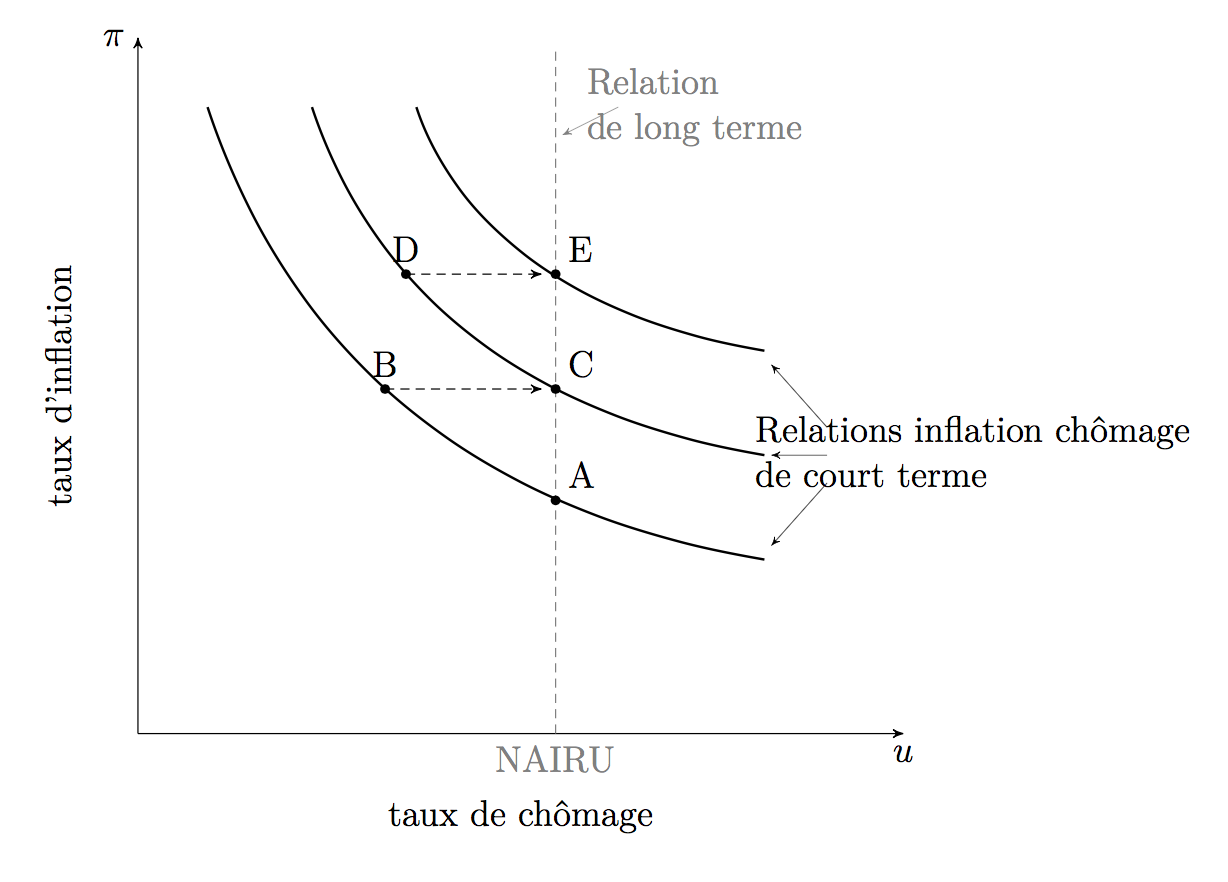
\includegraphics[scale=0.5]{./img/im3}
		
	\end{center}
	\caption{Courbe de Phillips}
  \label{fig:courbe_phillips}
\end{figure}
\newpage

Cependant ces règles sont parfois difficiles à assumer. Par exemple la stabilisation de l'inflation des années 80 a eu de fortes répercussions de croissance  en France, ainsi que l'implication d'une perte de l'avantage concurrentiel (dûe au faible prix des produits français en relation aux autres).

On définit plus tard des politiques globales à l'Europe: 
\begin{enumerate}
	\item Taux d'inflation <1.5$\%$ de la moyenne des membres le plus performants.
	\item Devise devant rester au moins 2 ans dans le système monétaire.
	\item Intérêt moyen et long terme <$2\%$ des pays les moins inflationnistes.
	\item Dette <$60\%$ du PIB.
	\item Déficit public <$3\%$ du PIB.
	
\end{enumerate}

Un ensemble de contraintes, qui se voient fortement contrastées par les temps de crise ( dette France $\approx$ 100$\%$ PIB).

On présente 2 principes importants pour analyser la situation de la zone Euro. 
\newline

\textbf{Règle de Taylor}: 	
\[
	\text{Taux d'intérêt}= f(\text{taux d'inflation-taux d'inflation cible},\text{taux de croissance-taux de croissance potentielle})
\]
\textbf{Mundell}: Seuls 2 des 3 objectifs suivants peuvent être atteints simultanéments: 
\begin{enumerate}
	\item Stabilité des changes.
	\item Liberté des mouvements des capitaux.
	\item Indépendance nationale des politiques monétaires. 
\end{enumerate}

La zone Euro à déjà obtenu la liberté de mouvement des capitaux, et ne s'impose pas de tendre vers une stabilité de l'euro par rapport au dollar. Cependant pour le
dernier point, il est complexe de mener une politique commune dans une zone si diverse. Selon Mundell \emph{l'Europe n'est pas une zone monétaire optimale}.
Les conditions seraient réunies si : 
\begin{itemize}
	\item Faible degré d'asymétrie entre les chocs subis par les différents pays.
	\item Mobilité importante des facteurs de production, pour amortir les chocs. 
\end{itemize}
Ces conditions ne sont clairements pas réunies en Europe (par exemple la situation de la Grèce pendant la crise).
% subsection politique_monetaire (end)
\subsection{La politique budgétaire} % (fold)
\label{sub:la_politique_budgetaire}
On introduit ci-dessous le modèle IS-LM, ce modèle considère que les leviers principaux pour faire varier la politique économique de l'État sont la politique 
budgétaire et la politique monétaire. La politique monétaire est gérée par la BCE il ne reste donc que la politique budgétaire aux États.

\begin{tcolorbox}[title= Modèle IS-LM] 
	Ce modèle se réfère à la mise en équation de la pensée Keynésienne, faite par Hicks (1937). C'est une analyse conjointe du marché de la monnaie et du marché des biens, en supposant les prix fixes (représentation court terme de l'équilibre macroéconomique). 
  On pose $Y=PIB=C+I+G$ avec $C$ la consommation, $I$ l'investissement privé, et $G$ l'investissement public. Les fonctions $I$ et $C$ vont varier en fonction de paramètres implicites au modèle :
	\begin{itemize}[label=\ding{69}]
		\item $C$ augmente avec les revenus mais diminue avec $r$.
		\item $I$ augmente avec les ventes courantes et diminue avec $r$.
	\end{itemize}
Pour comprendre ce modèle il faut penser que les images suivantes ne sont que des courbes de niveau, de fonctions à 2 variables. Représentant l'évolution 
de la courbe pour un niveau de satisfaction donné. On obtient ainsi les modèles suivants. 

	\begin{center}
		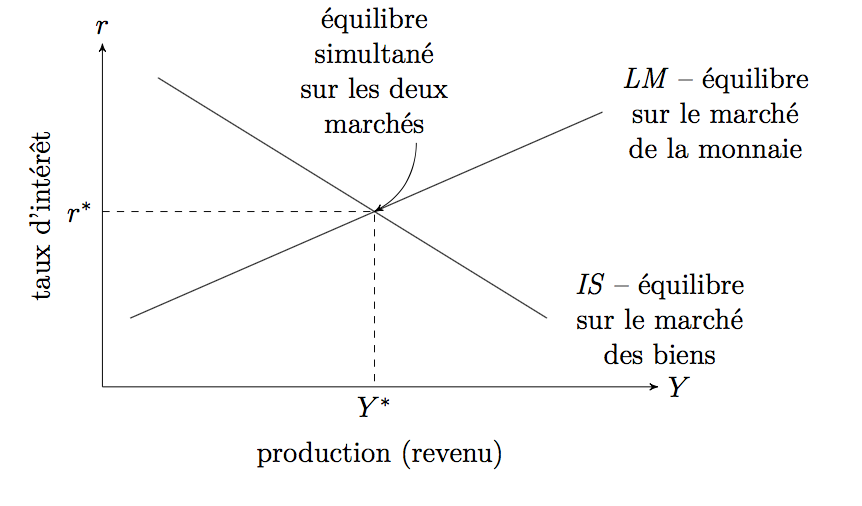
\includegraphics[scale=0.5]{./img/im4}
	\end{center}
	\captionof{figure}{Modèle IS-LM}
  \label{fig:modele_islm}

Suite aux influences implicites de certains paramètres et à l'analyse économique
on obtient ce modèle suite à deux politiques différentes:
la politique restrictive représentée à la figure~\ref{fig:modele_islm_rest}
et la politique expansioniste à la figure~\ref{fig:modele_islm_exp}.
\end{tcolorbox}

\begin{figure}[h]
		\begin{center}
			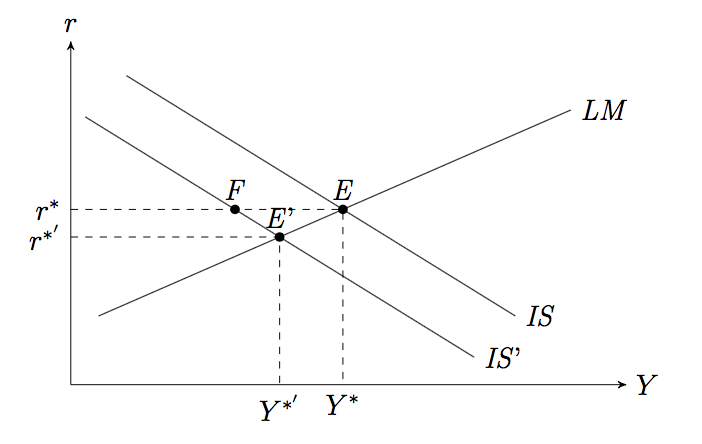
\includegraphics[scale=0.5]{./img/im5}
		\end{center}
		\caption{Modèle IS-LM avec une politique restrictive}
	   \label{fig:modele_islm_rest}
\end{figure}	
\begin{figure}[h]
		\begin{center}
			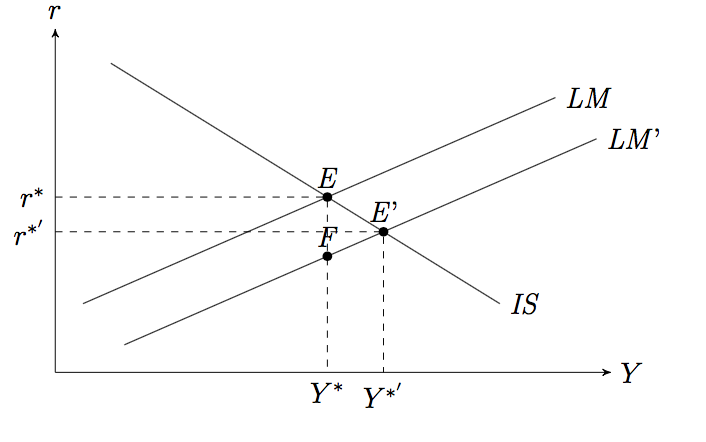
\includegraphics[scale=0.5]{./img/im6}
		\end{center}
		\caption{Modèle IS-LM politique monétaire expansionistes}
	   \label{fig:modele_islm_exp}
\end{figure}

L'Europe actuelle présente une faible marge de manoeuvre au niveau de la politique économique monétaire et budgétaire. Cette situation découle du contrôle de 
la politique monétaire par la BCE. On se retrouve dans une situation où l'on considère que les dépenses de l'État n'influencent pas le niveau de l'activité 
économique (pré-keynésienne). Aujourd'hui c'est même la hausse des demandes de l'État et des taux d'intérêts (pour investir sur le marché financier) qui est 
critiquée. Ces éléments impliquent un ralentissement des investissements et des achats financés par l'emprunt. Il convient de distinguer 2 politiques 
envisageables : 
\begin{itemize}[label=\ding{69}]
	\item Politique budgétaire contra-cyclique. Elle s'exerce afin d'atténuer les aléas de la conjoncture économique, en jouant sur la fiscalité et les 
	dépenses publiques. Par exemple, l'effet des dépenses publiques: elles vont accélerer quand l'activité économique s'affaiblit. Ceci va provoquer une 
	diminution des revenus fiscaux et donc des dépenses budgétaires. On dit que recettes et dépenses publiques agissent comme des \emph{stabilisateurs
	automatiques}.
	\item Politique budgétaire volontariste. Elle se base sur l'effet du \emph{multiplicateur keynésien} à court terme. On essaie de profiter de l'effet
	d'augmentation initiale du pouvoir d'achat pour créer de l'emploi, en créant des opportunités. 
\end{itemize}

% subsection la_politique_budgetaire (end)

\subsection{Le chômage} % (fold)
\label{sub:le_chomage}

Selon Keynes il est plus intéressant de favoriser la demande de travail que de baisser les salaires pour favoriser l'offre (en quantité).
Le chômage est modelé par les 2 forces suivantes : 
\begin{enumerate}
	\item \emph{Règle du côté court}, on ne peut obliger un agent à acheter un bien que s'il le désire au prix du marché. Donc l'entreprise ne produit que ce 
	qu'elle va vendre.
	\item Le chômage \emph{classique} souffre aussi d'un double désequilibre. Offre inférieure à la demande sur le marché des biens, (réduction de l'offre
	en raison des coûts de production élevés). Offre supérieure à la demande sur le marché des biens (demande de travail des firmes réduite de part 
	le coût de la main d'oeuvre).
\end{enumerate}

La persistance du chômage a un lien direct avec le salaire. pour analyser ce dernier on analyse 2 théories récentes : 
\begin{itemize}
	\item \emph{Salaire d'efficience}, c'est un salaire supérieur au salaire moyen pour inciter le salarié à travailler.
	\item \emph{Négociations salariales}, les syndicats essaient de faire augmenter le salaire et les conditions de travail, le revers de la négociation 
	est la création d'un chômage involontaire.
\end{itemize}
Depuis quelques années les politiques européennes en matière de chômage se basent sur un allègement de la fiscalité pour embaucher du personnel, afin 
de stimuler l'offre de travail.

On terminera la section en analysant le phénomène de \emph{trappe à pauvreté}. Ce concept se réfère à l'inertie que créent les minima sociaux, pour sortir de
la situation du chômage. Pour contrer ce phénomène on voit par exemple une prime de reprise d'emploi de 1000 euros en France.

% subsection le_chomage (end)
\subsection{L'endettement de l'État} % (fold)
\label{sub:l_endettement_de_l_etat}

L'État français est en déficit chaque année depuis 1975, les \emph{ pactes de stabilité et de croissance} se sont assouplis en 2005 (anticipant sans le savoir la crise).
Cependant que penser de la dette qu'accumulent les États de l'Union Européenne ? Si on calcule différents ratios on se rend compte que cette dette est 
difficilement soutenable. Cependant il faut l'interpréter dans la période actuelle de crise des comptes sociaux, il faut relativiser, en effet le patrimoine
est plus élevé (oeuvres d'art...). On doit tout de même être méfiants de l'avenir, dans lequel la population à la retraite augmente (babyboom années 30), ce qui va alourdir les dépenses de l'État.

La France a mis en place une politique qui se base sur la minimisation des dépenses dans certains secteurs ainsi qu'un grand prêt, pour favoriser la relance 
économique et les dépenses en éducation (pour apporter de l'innovation..). 

De plus la France s'inscrit dans la moyenne des pays vertueux de l'Union, il faut cependant s'inquiéter des fortes asymétries qui y existent.


% subsection l_endettement_de_l_etat (end)

% section conjoncture_et_politiques_economiques (end)
